\documentclass{report}
\usepackage{graphicx, tikz-cd, float, titlepic, booktabs} % Required for inserting images
\usepackage{pgfplots}
\usepackage{multicol}
\usepackage{makecell}
\pgfplotsset{compat=1.15}
\usepackage{mathrsfs}
\usetikzlibrary{arrows}
\usepackage{amsmath, amssymb, amsthm, amsfonts, siunitx, physics, gensymb}
\AtBeginDocument{\RenewCommandCopy\qty\SI}
\usepackage[version=4]{mhchem}
\usepackage[most,many,breakable]{tcolorbox}
\usepackage{xcolor, fancyhdr, varwidth}
\usepackage[Glenn]{fncychap}
%Options: Sonny, Lenny, Glenn, Conny, Rejne, Bjarne, Bjornstrup
\usepackage{hyperref, cleveref}
\usepackage{icomma, enumitem} %comma as decimal and continue enumerate with [resume]
\usepackage{plimsoll} %use standard state symbol with \stst
\usepackage[danish]{babel}
\usepackage{halloweenmath}
\renewcommand{\cellalign}{cl}
\renewcommand{\theadalign}{cl}
\renewcommand\theadfont{\bfseries}
%%%%%%%%%%%%%%%%%%%%%%%%%%%%%%
% SELF MADE COLORS
%%%%%%%%%%%%%%%%%%%%%%%%%%%%%%
\definecolor{myg}{RGB}{56, 140, 70}
\definecolor{myb}{RGB}{45, 111, 177}
\definecolor{myr}{RGB}{199, 68, 64}
\definecolor{mytheorembg}{HTML}{F2F2F9}
\definecolor{mytheoremfr}{HTML}{00007B}
\definecolor{mylenmabg}{HTML}{FFFAF8}
\definecolor{mylenmafr}{HTML}{983b0f}
\definecolor{mypropbg}{HTML}{f2fbfc}
\definecolor{mypropfr}{HTML}{191971}
\definecolor{myexamplebg}{HTML}{F2FBF8}
\definecolor{myexamplefr}{HTML}{88D6D1}
\definecolor{myexampleti}{HTML}{2A7F7F}
\definecolor{mydefinitbg}{HTML}{E5E5FF}
\definecolor{mydefinitfr}{HTML}{3F3FA3}
\definecolor{notesgreen}{RGB}{0,162,0}
\definecolor{myp}{RGB}{197, 92, 212}
\definecolor{mygr}{HTML}{2C3338}
\definecolor{myred}{RGB}{127,0,0}
\definecolor{myyellow}{RGB}{169,121,69}
\definecolor{myexercisebg}{HTML}{F2FBF8}
\definecolor{myexercisefg}{HTML}{88D6D1}
%%%%%%%%%%%%%%%%%%%%%%%%%%%%%%%%%%%%%%%%%%%%%%%%%%%%%%%%%%%%%%%%%%%%%%
% Box environments for theorems and problems
%%%%%%%%%%%%%%%%%%%%%%%%%%%%%%%%%%%%%%%%%%%%%%%%%%%%%%%%%%%%%%%%%%%%%
\setlength{\parindent}{1cm}
%================================
% Question BOX
%================================
\newtcbtheorem[]{question}{Opgave}{enhanced,
	before skip=2mm,after skip=2mm, colback=red!5,colframe=red!80!black,boxrule=0.5mm,
	attach boxed title to top left={xshift=1cm,yshift*=1mm-\tcboxedtitleheight}, varwidth boxed title*=-3cm,
	boxed title style={frame code={
					\path[fill=tcbcolback]
					([yshift=-1mm,xshift=-1mm]frame.north west)
					arc[start angle=0,end angle=180,radius=1mm]
					([yshift=-1mm,xshift=1mm]frame.north east)
					arc[start angle=180,end angle=0,radius=1mm];
					\path[left color=tcbcolback!60!black!65!red,right color=tcbcolback!60!black!65!red,
						middle color=tcbcolback!80!black!65!red!1!red]
					([xshift=-2mm]frame.north west) -- ([xshift=2mm]frame.north east)
					[rounded corners=1mm]-- ([xshift=1mm,yshift=-1mm]frame.north east)
					-- (frame.south east) -- (frame.south west)
					-- ([xshift=-1mm,yshift=-1mm]frame.north west)
					[sharp corners]-- cycle;
				},interior engine=empty,
		},
	fonttitle=\bfseries,
	title={#2},#1}{def}


\makeatletter
\newtcbtheorem{Question}{Opgave}{enhanced,
	breakable,
	colback=white,
	colframe=myb!80!black,
	attach boxed title to top left={yshift*=-\tcboxedtitleheight},
	fonttitle=\bfseries,
	title={#2},
	boxed title size=title,
	boxed title style={%
			sharp corners,
			rounded corners=northwest,
			colback=tcbcolframe,
			boxrule=0pt,
		},
	underlay boxed title={%
			\path[fill=tcbcolframe] (title.south west)--(title.south east)
			to[out=0, in=180] ([xshift=5mm]title.east)--
			(title.center-|frame.east)
			[rounded corners=\kvtcb@arc] |-
			(frame.north) -| cycle;
		},
	#1
}{def}
\makeatother
%================================
% DEFINITION BOX
%================================

\newtheorem{defin}{Definition}[section] % Creates a new counter, number within section

\newtcbtheorem[number within=section, use counter*=defin]{Definition}{Definition}{enhanced,
	before skip=2mm,after skip=2mm, colback=red!5,colframe=red!80!black,boxrule=0.5mm,
	attach boxed title to top left={xshift=1cm,yshift*=1mm-\tcboxedtitleheight}, varwidth boxed title*=-3cm,
	boxed title style={frame code={
					\path[fill=tcbcolback]
					([yshift=-1mm,xshift=-1mm]frame.north west)
					arc[start angle=0,end angle=180,radius=1mm]
					([yshift=-1mm,xshift=1mm]frame.north east)
					arc[start angle=180,end angle=0,radius=1mm];
					\path[left color=tcbcolback!60!black,right color=tcbcolback!60!black,
						middle color=tcbcolback!80!black]
					([xshift=-2mm]frame.north west) -- ([xshift=2mm]frame.north east)
					[rounded corners=1mm]-- ([xshift=1mm,yshift=-1mm]frame.north east)
					-- (frame.south east) -- (frame.south west)
					-- ([xshift=-1mm,yshift=-1mm]frame.north west)
					[sharp corners]-- cycle;
				},interior engine=empty,
		},
	fonttitle=\bfseries,
	title={#2},#1}{def}

\newtcbtheorem[number within=section]{definition}{Definition}
{%
	enhanced,
	breakable,
	colback = red!5,
	frame hidden,
	boxrule = 0sp,
	borderline west = {2pt}{0pt}{solid, red!75!black},
	sharp corners,
	detach title,
	before upper = \tcbtitle\par\smallskip,
	coltitle = red!75!black,
	fonttitle = \bfseries\sffamily,
	description font = \mdseries,
	separator sign none,
	segmentation style={solid, red!75!black},
}
{th}

\newtcbtheorem{theo}%
    {Theorem}{}{theorem}
\newtcolorbox{prob}[1]{colback=red!5!white,colframe=red!50!black,fonttitle=\bfseries,title={#1}}

%================================
% NOTE BOX
%================================

\usetikzlibrary{arrows,calc,shadows.blur}
\tcbuselibrary{skins}
\newtcolorbox{note}[1][]{%
	enhanced jigsaw,
	colback=gray!20!white,%
	colframe=gray!80!black,
	size=small,
	boxrule=1pt,
	title=\textbf{Note:},
	halign title=flush center,
	coltitle=black,
	breakable,
	drop shadow=black!50!white,
	attach boxed title to top left={xshift=1cm,yshift=-\tcboxedtitleheight/2,yshifttext=-\tcboxedtitleheight/2},
	minipage boxed title=1.5cm,
	boxed title style={%
			colback=white,
			size=fbox,
			boxrule=1pt,
			boxsep=2pt,
			underlay={%
					\coordinate (dotA) at ($(interior.west) + (-0.5pt,0)$);
					\coordinate (dotB) at ($(interior.east) + (0.5pt,0)$);
					\begin{scope}
						\clip (interior.north west) rectangle ([xshift=3ex]interior.east);
						\filldraw [white, blur shadow={shadow opacity=60, shadow yshift=-.75ex}, rounded corners=2pt] (interior.north west) rectangle (interior.south east);
					\end{scope}
					\begin{scope}[gray!80!black]
						\fill (dotA) circle (2pt);
						\fill (dotB) circle (2pt);
					\end{scope}
				},
		},
	#1,
}
%================================
% EXAMPLE BOX
%================================
\newtcbtheorem[number within=section, use counter from=definition]{Example}{Example}
{%
	colback = myexamplebg
	,breakable
	,colframe = myexamplefr
	,coltitle = myexampleti
	,boxrule = 1pt
	,sharp corners
	,detach title
	,before upper=\tcbtitle\par\smallskip
	,fonttitle = \bfseries
	,description font = \mdseries
	,separator sign none
	,description delimiters parenthesis
}
{ex}
%================================
% THEOREM BOX
%================================

\tcbuselibrary{theorems,skins,hooks}
\newtcbtheorem[number within=section, use counter from=definition]{Theorem}{Theorem}
{%
	enhanced,
	breakable,
	colback = mytheorembg,
	frame hidden,
	boxrule = 0sp,
	borderline west = {2pt}{0pt}{mytheoremfr},
	sharp corners,
	detach title,
	before upper = \tcbtitle\par\smallskip,
	coltitle = mytheoremfr,
	fonttitle = \bfseries\sffamily,
	description font = \mdseries,
	separator sign none,
	segmentation style={solid, mytheoremfr},
}
{th}

%%%%%%%%%%%%%%%%%%%%%%%%%%%%%%%%%%%%%%%%%%%%%%%%%%%%%%%%%%%%%%%%%
% SELF MADE COMMANDS
%%%%%%%%%%%%%%%%%%%%%%%%%%%%%%
\newcommand{\sol}{\setlength{\parindent}{0cm}\textbf{\textit{Løsning:}}\setlength{\parindent}{1cm}}
%%%%%%%%%%%%%%%%%%%%%%%%%%%%%%%%%
\usepackage[tmargin=2cm,rmargin=1in,lmargin=1in,margin=0.85in,bmargin=2cm,footskip=.2in]{geometry}\pagestyle{fancy}
\lhead{Minrui Kevin Zhou 3.b $\bigpumpkin$}
\rhead{Elektriske køretøjer $\mathghost$}

\title{
\[
\mathwitch*
\]
Elektriske køretøjer\\
{\Large \textbf{3.b fysik A}}}
\author{Kevin Zhou}
\date{\today}

\begin{document}
\maketitle
\begin{note}
  Databog fysik kemi (2007) er benyttet ved beregningerne. $\mathbat$
\end{note}
\begin{question}{Elfærge}{}
  Batteriet på elfærgen Aurora har det maksimale energiindhold 4160 kWh.
Mens færgen er i havn, oplades batteriet i 7,5 minutter med effekten 10,5
MW.
Spændingsfaldet under opladningen er det samme som batteriets nominelle
spændingsfald.
\begin{itemize}
  \item[a.] Beregn ændringen i batteriets ladningstilstand under opladningen.
\end{itemize}
Færgens batteri er opbygget af en række parallelkoblede strenge, hvor hver
streng består af 192 seriekoblede elementer. Hvert element har
hvilespændingen 3,9 V.
Under sejlads aflades batteriet med strømstyrken 112 A, og nyttevirkningen
af batteriet er 98 \%.
\begin{itemize}
  \item[b.] Bestem den indre resistans i færgens batteri.
\end{itemize}
\end{question}
\sol \\
\textbf{a.}
Siden effekten $P$ er konstant under opladningen, så må ændringen i ladningstilstand være 
\begin{equation*}
\begin{split}
  \Delta SoC&=\frac{P \cdot \Delta t}{E _{\text{max} }}\\
  &=\frac{10,5 \cdot 10^6 \;\unit{W} \cdot 7,5 \;\unit{min} }{4160 \cdot 10^3 \;\unit{W} \cdot 60 \;\unit{min} }\\
  &\approx 0,32\\
  &=32 \%.
\end{split}
\end{equation*}
Ændringen i batteriets ladningstilstand under opladningen må da være 32 \%.\\[1ex]
\textbf{b.}
Siden strengene af seriekoblede elementer er parallelkoblede, så må der gælde, at den samlede hvilespænding må være
\begin{equation*}
\begin{split}
  U_0&=U_0(\text{streng 1}) = U_0(\text{streng 2}) = \cdots =U_0(\text{streng } n)\\
  &=192 \cdot 3,9 \;\unit{V},
\end{split}
\end{equation*}
fordi hver streng består af 192 seriekoblede elementer, der hver har hvilespænding på 3,9 V.

Imidlertid har vi, at
\begin{equation*}
\begin{split}
  \eta =1-\frac{R_i \cdot I}{U_0} \iff R_i =\frac{(1-\eta) \cdot U_0}{I}.
\end{split}
\end{equation*}
Vi indsætter da de kendte værdier og får
\begin{equation*}
\begin{split}
  R_i &=\frac{(1-\eta) \cdot U_0}{I}\\
  &=\frac{(1-0,98)\cdot 192 \cdot 3,9 \;\unit{V} }{112 \;\unit{A} }\\
  &\approx 0,13 \;\unit{\ohm}. 
\end{split}
\end{equation*}
Den indre resistans i færgens batteri er altså $0,13 \;\unit{\ohm}$.

\begin{question}{Opladning af batteri}{}
Et batteri har den indre modstand $0,090 \;\unit{\ohm}$ og hvilespændingen 4,2 V.
\begin{itemize}
  \item[a.] Beregn den maksimale effekt, hvormed batteriet kan afgive energi under afladning.
\end{itemize}
Under opladning af et helt afladet batteri måles strømstyrken $I$ igennem
batteriet som funktion af tiden $t$.
Efter 2,5 h er batteriet fuldt opladet.
\begin{itemize}
  \item[b.] Bestem den tid, det tager at oplade batteriet til ladningstilstanden 90 \%.
\end{itemize}
\end{question}
\sol \\
\textbf{a.}
Den maksimale effekt må være
\begin{equation*}
\begin{split}
  P _{\text{max} }&=\frac{U_0^2}{4 \cdot R_i}\\
  &=\frac{\left(4,2 \;\unit{V} \right) ^2}{4 \cdot 0,090 \;\unit{\ohm}}\\
  &=49 \;\unit{W}.
\end{split}
\end{equation*}
Den maksimale effekt, hvormed batteriet kan afgive energi under afladning er altså $49 \;\unit{W}$.\\[1ex]
\textbf{b.}
Der gælder, at
\[
\Delta Q= \int_{t_1}^{t_2} I \,dt. 
\] 
Vi indsætter derfor de givne data i Logger Pro og finder arealet under $(t, I)$-grafen fra $t=0 \;\unit{h} $ til $t=2,5 \;\unit{h}$, som må svare til batteriets maksimale ladningskapacitet $Q _{\text{max} }$ (se \cref{fig:batteri}).
Vi får fra den numeriske integration, at
\[
Q _{\text{max} }=0,8042 \;\unit{A \cdot h}.
\] 
Vi kan nu udregne, hvilken ladningsmængde $Q_t$ batteriet har, når $SoC_t=90 \%$:
\begin{equation*}
\begin{split}
  Q_t &= SoC_t \cdot Q _{\text{max} }\\
  &= 0,9 \cdot 0,8042 \;\unit{A \cdot h} \\
  &\approx 0,7238 \;\unit{A \cdot h}. 
\end{split}
\end{equation*}
Fra \cref{fig:batteri} ser vi, at dette netop er tilfældet, når $t=1,04 \;\unit{h}$.
Altså tager det $1,04 \;\unit{h}$ at oplade batteriet til ladningstilstanden 90 \%.
\begin{figure}[H]
\begin{center}
  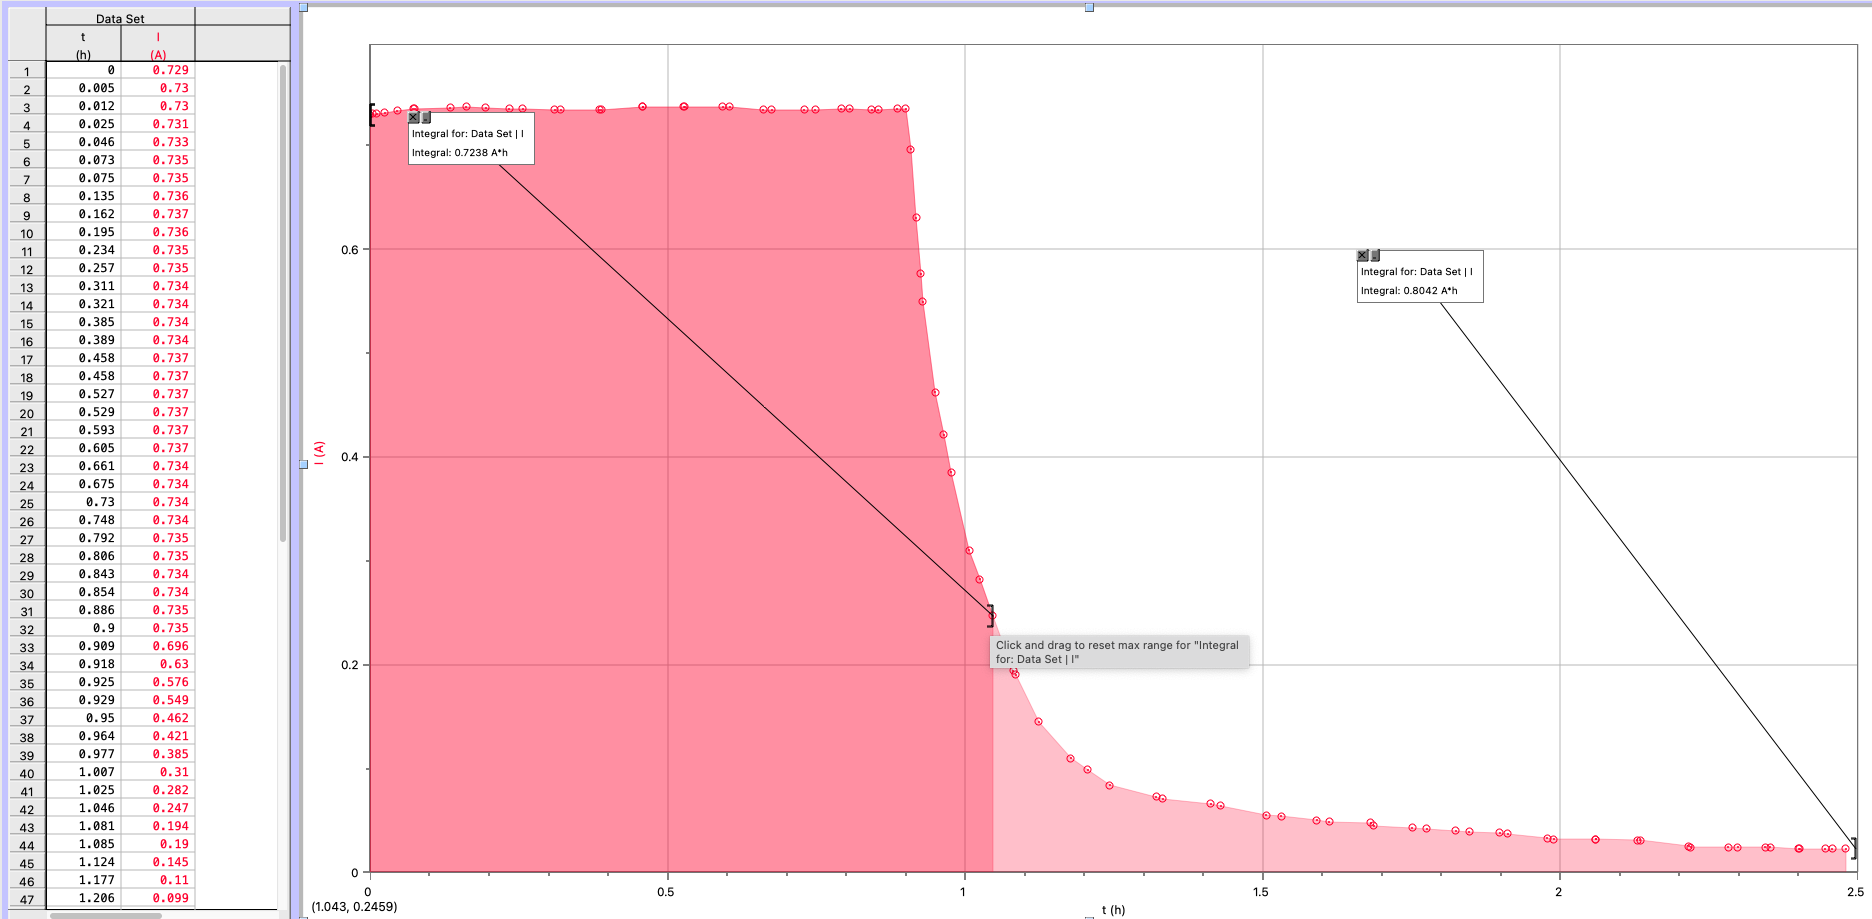
\includegraphics[width=0.8\textwidth]{batteri.png}
\end{center}
  \caption{Numerisk integration på $(t,I)$-grafen}
\label{fig:batteri}
\end{figure}

\begin{question}{Elektrisk rallybil}{}
  Under kørslen i en elektrisk rallybil afsættes energi i elektromotorens vindinger med effekten 2,08 kW.
  Vindingsresistansen i motoren er $12 \;\unit{m\ohm}$.
  \begin{itemize}
    \item[a.] Beregn strømstyrken igennem elektromotorens vindinger.
  \end{itemize}
Elektromotoren forsynes med spændingsfaldet 100 V, og strømstyrken igennem motoren er 416 A. Motorkonstanten er 0,46 Vs.
\begin{itemize}
  \item[b.] Bestem motorens omdrejningstal, og bestem motorens mekaniske effekt.
\end{itemize}
\end{question}
\sol \\
\textbf{a.}
Lad $R_0$ betegne vindingsresistansen i motoren.
Et udtryk for strømstyrken gennem vindingerne må være
\begin{equation*}
\begin{split}
P=R_0 \cdot I^2 \iff I=\sqrt{\frac{P}{R_0}}.
\end{split}
\end{equation*}
Vi indsætter de kendte værdier, og udregner $I$.
\begin{equation*}
\begin{split}
  I&=\sqrt{\frac{P}{R_0}}\\
  &=\sqrt{\frac{2,08 \cdot 10^3 \;\unit{W} }{12 \cdot 10 ^{-3} \;\unit{\ohm} }} \\
  &\approx 4,2 \cdot 10^2 \;\unit{A}.
\end{split}
\end{equation*}
Strømstyrken igennem elektromotorens vindinger er altså $4,2 \cdot 10^2 \;\unit{A} $. \\[1ex]
\textbf{b.}
Vi starter med at finde et udtryk for det inducerede spændingsfald $U_m$.
\begin{equation*}
\begin{split}
  U=R_0 \cdot I + U_m \iff U_m=U-R_0 \cdot I,
\end{split}
\end{equation*}
hvor $U$ er forsyningsspændingen. 
Vi kan nu finde et udtryk for motorens frekvens:
\begin{equation*}
\begin{split}
  U_m=K \cdot \omega &\iff \omega =\frac{U_m}{K}\\
  &\iff f =\frac{U-R_0 \cdot I}{K \cdot 2 \pi }.
\end{split}
\end{equation*}
Vi indsætter da de kendte værdier og udregner frekvensen til at være
\begin{equation*}
\begin{split}
  f &=\frac{U-R_0 \cdot I}{K \cdot 2 \pi }\\
  &=\frac{100 \;\unit{V} - 12 \cdot 10 ^{-3} \;\unit{\ohm} \cdot 416 \;\unit{A} }{0,46 \;\unit{V \cdot s} \cdot 2 \pi }\\
  &\approx 33 \;\unit{Hz}\\
  &\approx 2,0 \cdot 10^3 \;\unit{min ^{-1}}.
\end{split}
\end{equation*}
Det vil altså sige, at motoren har et omdrejningstal på $2,0 \cdot 10^3 \;\unit{rpm}$.

Imidlertid har vi, at motorens mekaniske effekt må være
\begin{equation*}
\begin{split}
  P _{\text{mek} }&=M \cdot \omega \\
  &=K \cdot I \cdot \frac{U-R_0 \cdot I}{K}\\
  &=I \cdot \left(U-R_0 \cdot I\right) \\
  &=416 \;\unit{A} \cdot \left(100 \;\unit{V} - 12 \cdot 10 ^{-3} \;\unit{\ohm} \cdot 416 \;\unit{A} \right) \\
  &\approx 4,0 \cdot 10^4 \;\unit{W} \\
  &=40 \;\unit{kW}.
\end{split}
\end{equation*}
Motorens mekaniske effekt er altså $40 \;\unit{kW} $.

\begin{question}{Motor til elcykel}{}
  Når motoren står stille, og spændingsfaldet over motoren er 1,05 V, er strømstyrken igennem motoren $0,66 \;\unit{A}$.
  \begin{itemize}
    \item[a.] Beregn motorens vindingsresistans.
  \end{itemize}
Ved et eksperiment måles sammenhørende værdier for motorens moment $M$  og strømstyrken $I$ igennem motoren.
Bilaget Elcykel indeholder data fra eksperimentet.
Motorens nyttevirkning er størst ved 1002 omdrejninger pr. minut, hvor strømstyrken igennem motoren er 6,99 A, og spændingsfaldet over motoren er 42,2 V.
\begin{itemize}
  \item[b.] Brug bilaget til at bestemme motorkonstanten for elmotoren. Beregn motorens største nyttevirkning.
\end{itemize}
\end{question}
\sol \\
\textbf{a.}
Siden motoren står stille, så må det inducerede spændingsfald være 0, og vindingsresistansen bliver derfor
\begin{equation*}
\begin{split}
  R_0&=\frac{U}{I}\\
  &=\frac{1,05 \;\unit{V} }{0,66 \;\unit{A} }\\
  &\approx 1,6 \;\unit{\ohm}.
\end{split}
\end{equation*}
Motorens vindingsresistans er altså $1,6 \;\unit{\ohm}$.\\[1ex]
\textbf{b.}
Der gælder for en motors kraftmoment, at
\begin{equation}
\label{eq:moment} 
M=K \cdot I,
\end{equation}
hvor $K$ er motorkonstanten. 
Altså må punkterne på $(I, M)$-grafen ligge på en ret linje gennem (0,0) med en hældning på $K$.
Vi laver derfor en ligefrem proportional regression på $(I, M)$-grafen, hvilket ses i \cref{fig:IM}.
\begin{figure}[H]
\begin{center}
  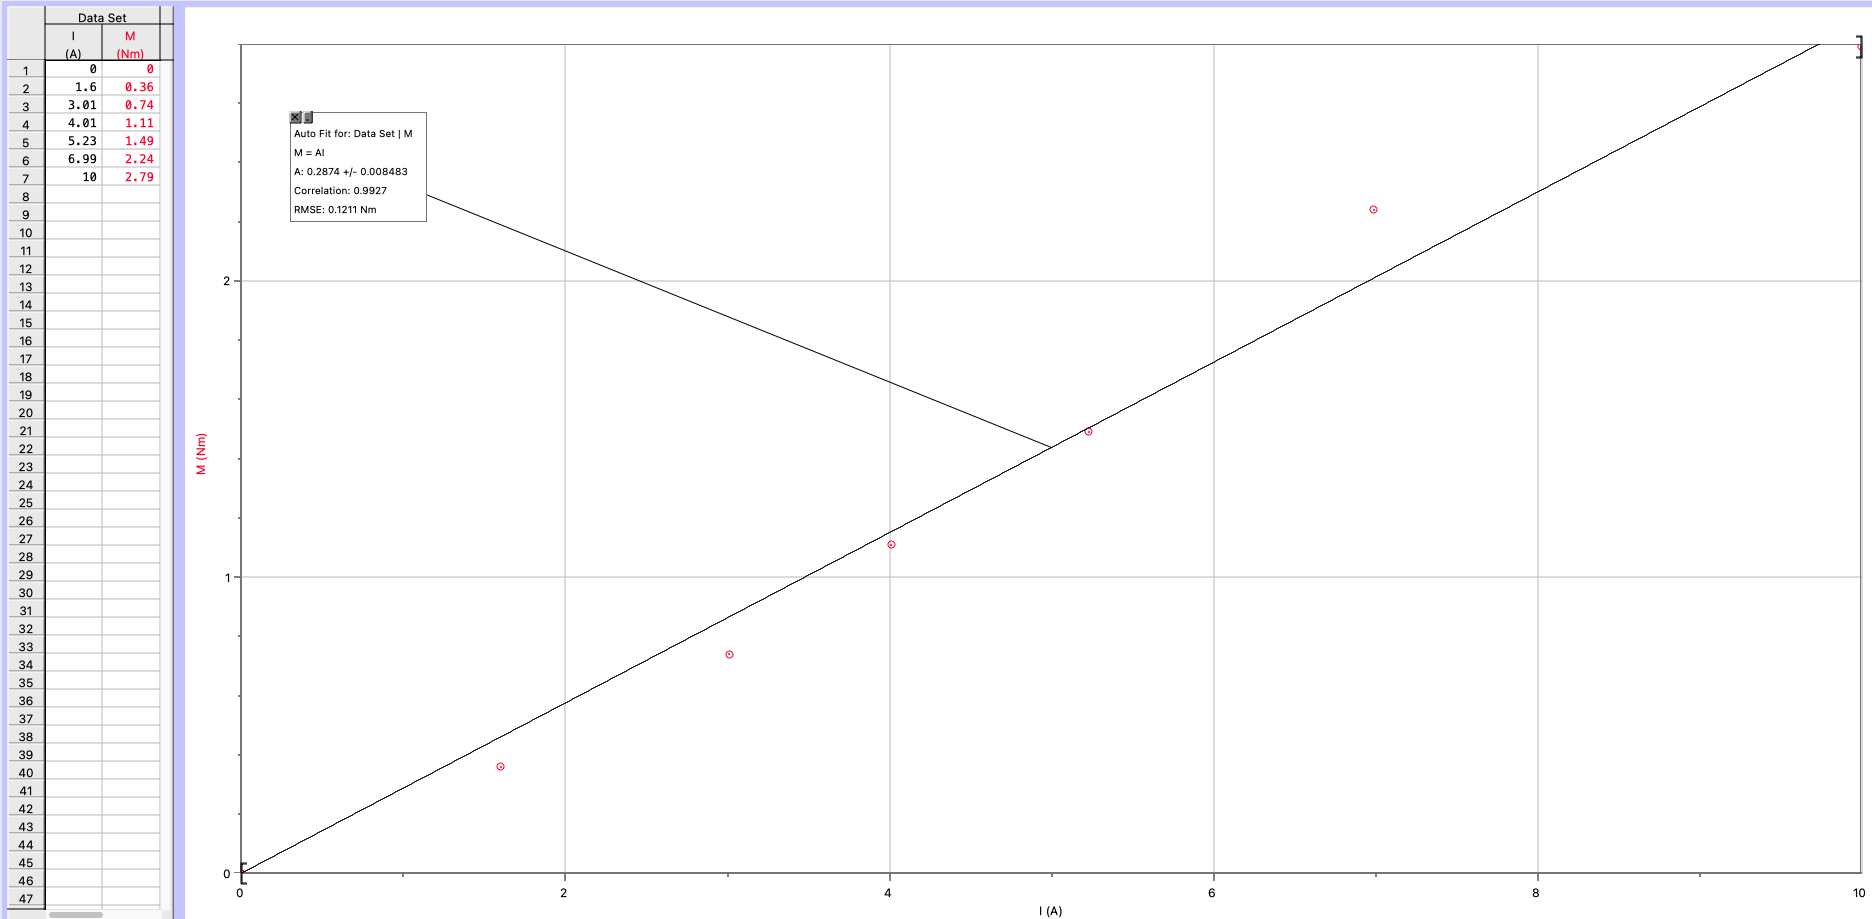
\includegraphics[width=0.8\textwidth]{IM.png}
\end{center}
  \caption{Regression på $(I, M)$-grafen}
\label{fig:IM}
\end{figure}
Det ses som forventet, at punkterne tilnærmelsesvist ligger på en ret linje gennem (0,0).
Fra regressionen har vi, at 
\[
M=0,287 \;\unit{V \cdot s} \cdot I.
\] 
Sammenligner vi med ligning (\ref{eq:moment}), er det klart, at motorkonstanten for elmotoren må være $2,387 \;\unit{V \cdot s}$.

Vi beregner nu motorens største nyttevirkning, som må være
\begin{equation*}
\begin{split}
  \eta &=1-\frac{M \cdot R_0}{K \cdot U}\\
  &=1- \frac{I \cdot R_0}{U}\\
  &=1-\frac{6,99 \;\unit{A} \cdot 1,5909 \;\unit{\ohm} }{42,2 \;\unit{V}}\\
  &\approx 0,736.
\end{split}
\end{equation*}
Motorens største nyttevirkning er altså $0,736$.

\begin{question}{Elfærgen Ellen}{}
  Elfærgens batteri indeholder den tilgængelige energi 4,3 MWh, når det er fuldt opladet.
  Når færgen sejler med farten 25,7 km/h, omsætter motorerne elektrisk energi med effekten 1000 kW.
  \begin{itemize}
    \item[a.] Vurdér, hvor langt elfærgen maksimalt kan sejle med farten 25,7 km/h.
  \end{itemize}
  Ved færgens ankomst til en havn er batteriets ladningstilstand 23 \%.
I havnen oplades batteriet i 30 minutter med strømstyrken 4,8 kA.
Batteriets nominelle spændingsfald er 750 V.
\begin{itemize}
  \item[b.] Beregn batteriets ladningstilstand efter opladningen.
\end{itemize}
\end{question}
\sol \\
\textbf{a.}
Siden der gælder, at $t=\frac{E}{P}$, så må den maksimale afstand, som færgen kan sejle, være
\begin{equation*}
\begin{split}
  s&=v \cdot t \\
  &=v \cdot \frac{E}{P}\\
  &=25,7 \;\unit{km/h} \cdot \frac{4,3 \cdot 10^6\;\unit{Wh}}{1000 \cdot 10^3 \;\unit{W}}\\
  &\approx 1,1 \cdot 10^2 \;\unit{km}.
\end{split}
\end{equation*}
Elfærgen kan altså maksimalt sejle $1,1 \cdot 10^2 \;\unit{km} $ med farten $25,7 \;\unit{km/h} $. \\[1ex]
\textbf{b.}
Fra sammenhængen mellem energiindholdet af et batteri og det nominelle spændingsfald har vi, at
\begin{equation*}
\begin{split}
  E _{\text{max} }=U _{\text{nom} } \cdot Q _{\text{max} } \iff Q _{\text{max} }=\frac{E _{\text{max} }}{U _{\text{nom} }}.
\end{split}
\end{equation*}
Efter opladningen må ladningstilstanden da være
\begin{equation*}
\begin{split}
  SoC _{\text{efter} }&=SoC _{\text{før} } + \frac{I \cdot \Delta t}{Q _{\text{max} }}\\
  &=SoC _{\text{før} } + \frac{I \cdot \Delta t \cdot U _{\text{nom} }}{E _{\text{max} }}\\
  &=0,23 + \frac{4,8 \cdot 10^3 \;\unit{A} \cdot 30 \cdot 60 \;\unit{s} \cdot 750 \;\unit{V} }{4,3 \cdot 10^6 \;\unit{W} \cdot 3600 \;\unit{s} }\\
  &\approx 0,65\\
  &= 65 \%.
\end{split}
\end{equation*}
Batteriets ladningstilstand efter opladningen er altså $65 \%$.

\begin{question}{Rekuperation}{}
  En elektromotor i en Renault Clio forsynes fra et batteri.
  Ved en fuld opladning er den maksimalt tilgængelige energi i batteriet 10,5 kWh, når det aflades under normale forhold.
  Den tilgængelige ladningskapacitet er 100 Ah.
  \begin{itemize}
    \item[a.] Beregn batteriets nominelle spændingsfald.
  \end{itemize}
Bilen har regenererende bremser, hvilket betyder, at strømmen under bremsning skifter retning og løber ind i batteriet, hvorved det oplades lidt.
Grafen viser belastningsstrømmen fra batteriet under en kørsel, hvor der bremses et par gange.
\begin{itemize}
  \item[b.] Beregn ændringen i ladningstilstanden for batteriet under kørslen
\end{itemize}
\end{question}
\sol \\
\textbf{a.}
Batteriets nominelle spændingsfald må være
\begin{equation*}
\begin{split}
  U _{\text{nom} }&=\frac{E _{\text{max} }}{Q _{\text{max} }}\\
  &=\frac{10,5 \cdot 10^3 \;\unit{Wh} }{100 \;\unit{Ah} }\\
  &=105 \;\unit{V}.
\end{split}
\end{equation*}
Batteriets nominelle spændingsfald er altså $105 \;\unit{V} $. \\[1ex]
\textbf{b.}
Siden vi har 
\begin{equation*}
\begin{split}
  \Delta Q = -\int_{t_1}^{t_2} I \,dt,
\end{split}
\end{equation*}
så kan vi finde ændringen i ladningen ved at tælle antallet af tern mellem $(t,I)$-grafen og førsteaksen (numerisk integration), hvilket ses i \cref{fig:rekup}.
\begin{figure}[H]
\begin{center}
  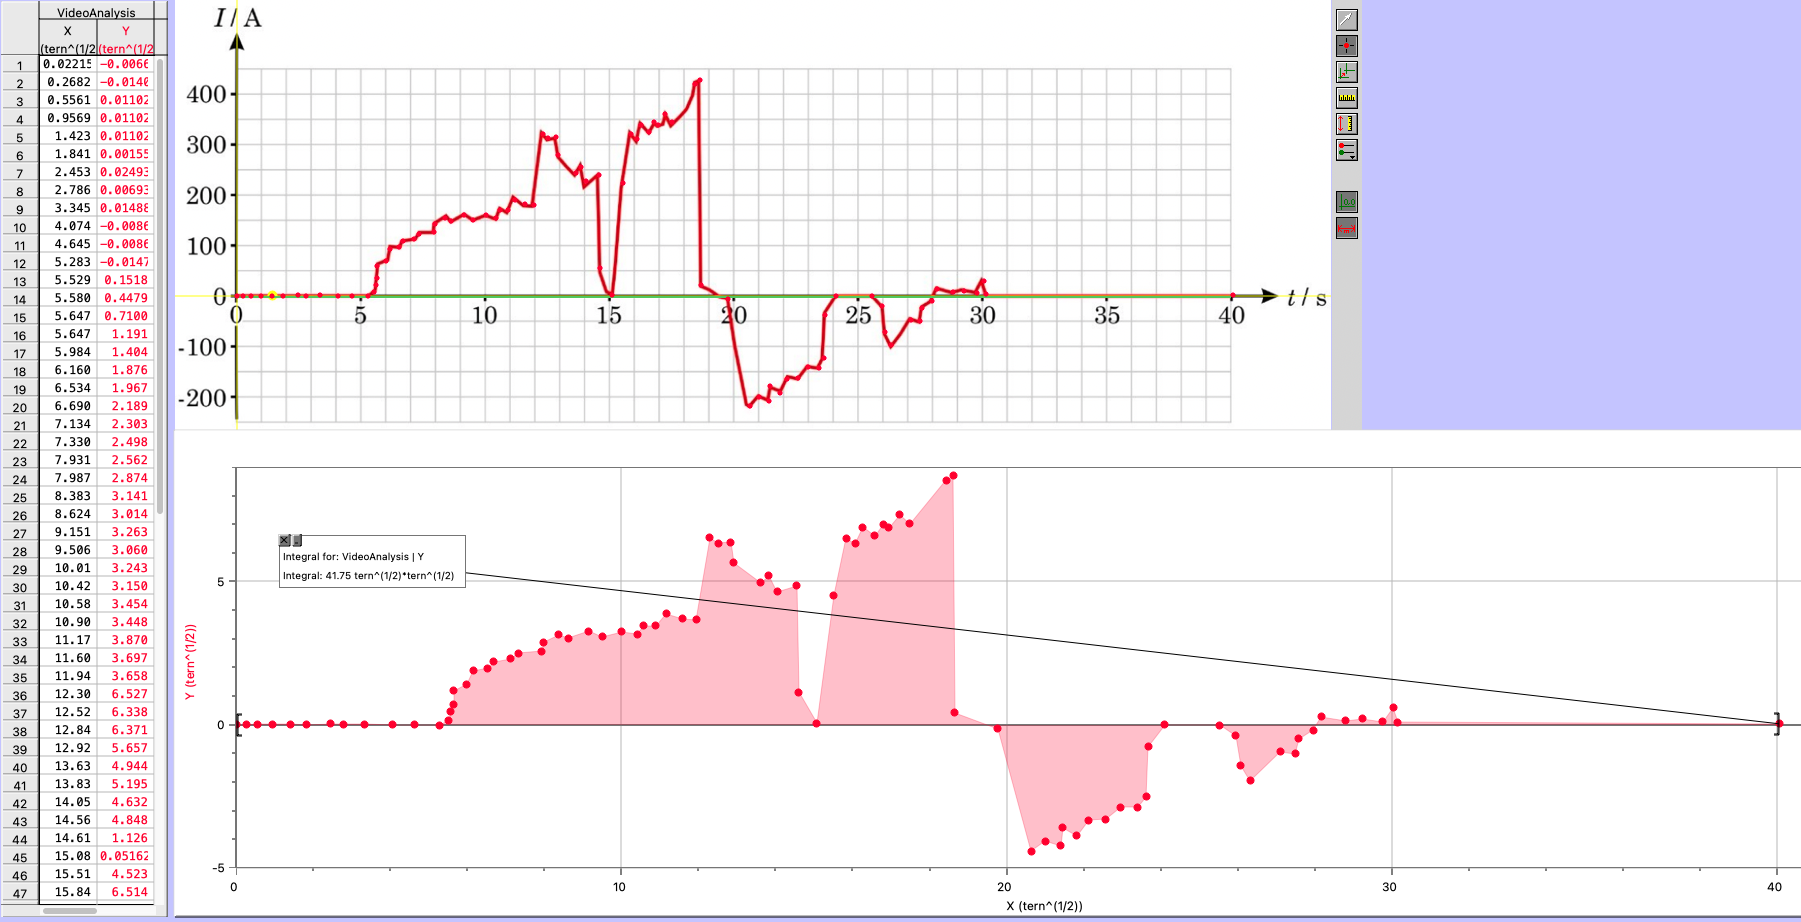
\includegraphics[width=0.8\textwidth]{rekup.png}
\end{center}
\caption{Numerisk integration af $(t, I)$-grafen}
\label{fig:rekup}
\end{figure}
Ændringen af ladningen fås til $41,75$ tern.
Imidlertid svarer hvert tern til 
\[
50 \;\unit{A} \cdot 1 \;\unit{s} =\frac{1}{72} \;\unit{A \cdot h}.
\] 
Ændringen i ladningstilstanden bliver da
\begin{equation*}
\begin{split}
  \Delta SoC &= \frac{\Delta Q}{Q _{\text{max} }}\\
  &=\frac{-41,75 \cdot \frac{1}{72} \;\unit{A \cdot h} }{100 \;\unit{A \cdot h} }\\
  &\approx -0,00580\\
  &=-0,580 \%.
\end{split}
\end{equation*}
Ændringen i ladningstilstanden for batteriet under kørslen er altså $-0,580 \%$.

\begin{question}{Kia Niro EV1}{}
  Med en hurtigoplader kan batteriet i en Kia Niro EV oplades fra 10 \% til 80 \% ladningstilstand på 41,0 minutter.
Den maksimalt tilgængelige kapacitet i batteriet er 181 Ah.
Opladningen sker med konstant strømstyrke.
\begin{itemize}
  \item[a.] Beregn størrelsen af strømstyrken ved en hurtigopladning.
\end{itemize}
Grafen viser størrelsen af elektromotorens moment som funktion af motorens omdrejningstal.
Under en kørsel leverer motoren en fremdriftskraft med størrelsen 6,8 kN.
Gearingsforholdet imellem motor og hjul er 10,65, og hjulenes radius er 0,334 m.
\begin{itemize}
  \item[b.] Beregn bilens fart under kørslen.
\end{itemize}
\end{question}
\sol \\
\textbf{a.}
Vi finder først et udtryk for strømstyrken ved opladningen.
\begin{equation*}
\begin{split}
  SoC _{\text{efter} }=SoC _{\text{før} } + \frac{I \cdot \Delta t}{Q _{\text{max} }} \iff I=\frac{Q _{\text{max} } \cdot \left(SoC _{\text{efter} }- SoC _{\text{før} }\right) }{\Delta t}.
\end{split}
\end{equation*}
Vi indsætter da de kendte værdier og udregner $I$, som er
\begin{equation*}
\begin{split}
  I&=\frac{Q _{\text{max} } \cdot \left(SoC _{\text{efter} }- SoC _{\text{før} }\right) }{\Delta t} \\
  &=\frac{181 \;\unit{A} \cdot 60 \;\unit{min} \cdot \left(0,80-0,10\right) }{41,0 \;\unit{min}}\\
  &\approx 1,9 \cdot 10^2 \;\unit{A}.
\end{split}
\end{equation*}
Størrelsen af strømstyrken ved en hurtigopladning er altså $1,9 \cdot 10^2 \;\unit{A} $.\\[1ex]
\textbf{b.}
Vi finder først et udtryk for motorens moment $M$ under kørslen. 
\begin{equation*}
\begin{split}
  F _{\text{frem} }= i \cdot \frac{M}{r _{\text{hjul} }} \iff M=\frac{F _{\text{frem} } \cdot r _{\text{hjul} }}{i},
\end{split}
\end{equation*}
hvor $i$ er gearingsforholdet. 
Vi udregner nu motorens moment $M$ under kørslen. 
\begin{equation*}
\begin{split}
  M&=\frac{F _{\text{frem} } \cdot r _{\text{hjul} }}{i}\\
  &=\frac{6,8 \cdot 10^3 \;\unit{N} \cdot 0,334 \;\unit{m} }{10,65}\\
  &\approx 213 \;\unit{Nm}.
\end{split}
\end{equation*}
Motorens omdrejningstal kan da aflæses på grafen, hvilket ses i \cref{fig:fM}.
Denne aflæses til at være 6650 omdrejninger pr. minut.
Vi kan nu udregne bilens fart under kørslen, som må være
\begin{equation*}
\begin{split}
  v&= \omega _{\text{hjul} } \cdot r \\
  &=\frac{\omega _{\text{motor} }}{i } \cdot r \\
  &=\frac{2 \pi \cdot f \cdot r}{i }\\
  &=\frac{2 \pi \cdot 6650 \cdot \left(60 \;\unit{s} \right) ^{-1}\cdot 0,334 \;\unit{m} }{10,65}\\
  &\approx 22 \;\unit{m/s}.
\end{split}
\end{equation*}
Bilens fart under kørslen er altså $22 \;\unit{m/s} $.

\begin{figure}[H]
\begin{center}
  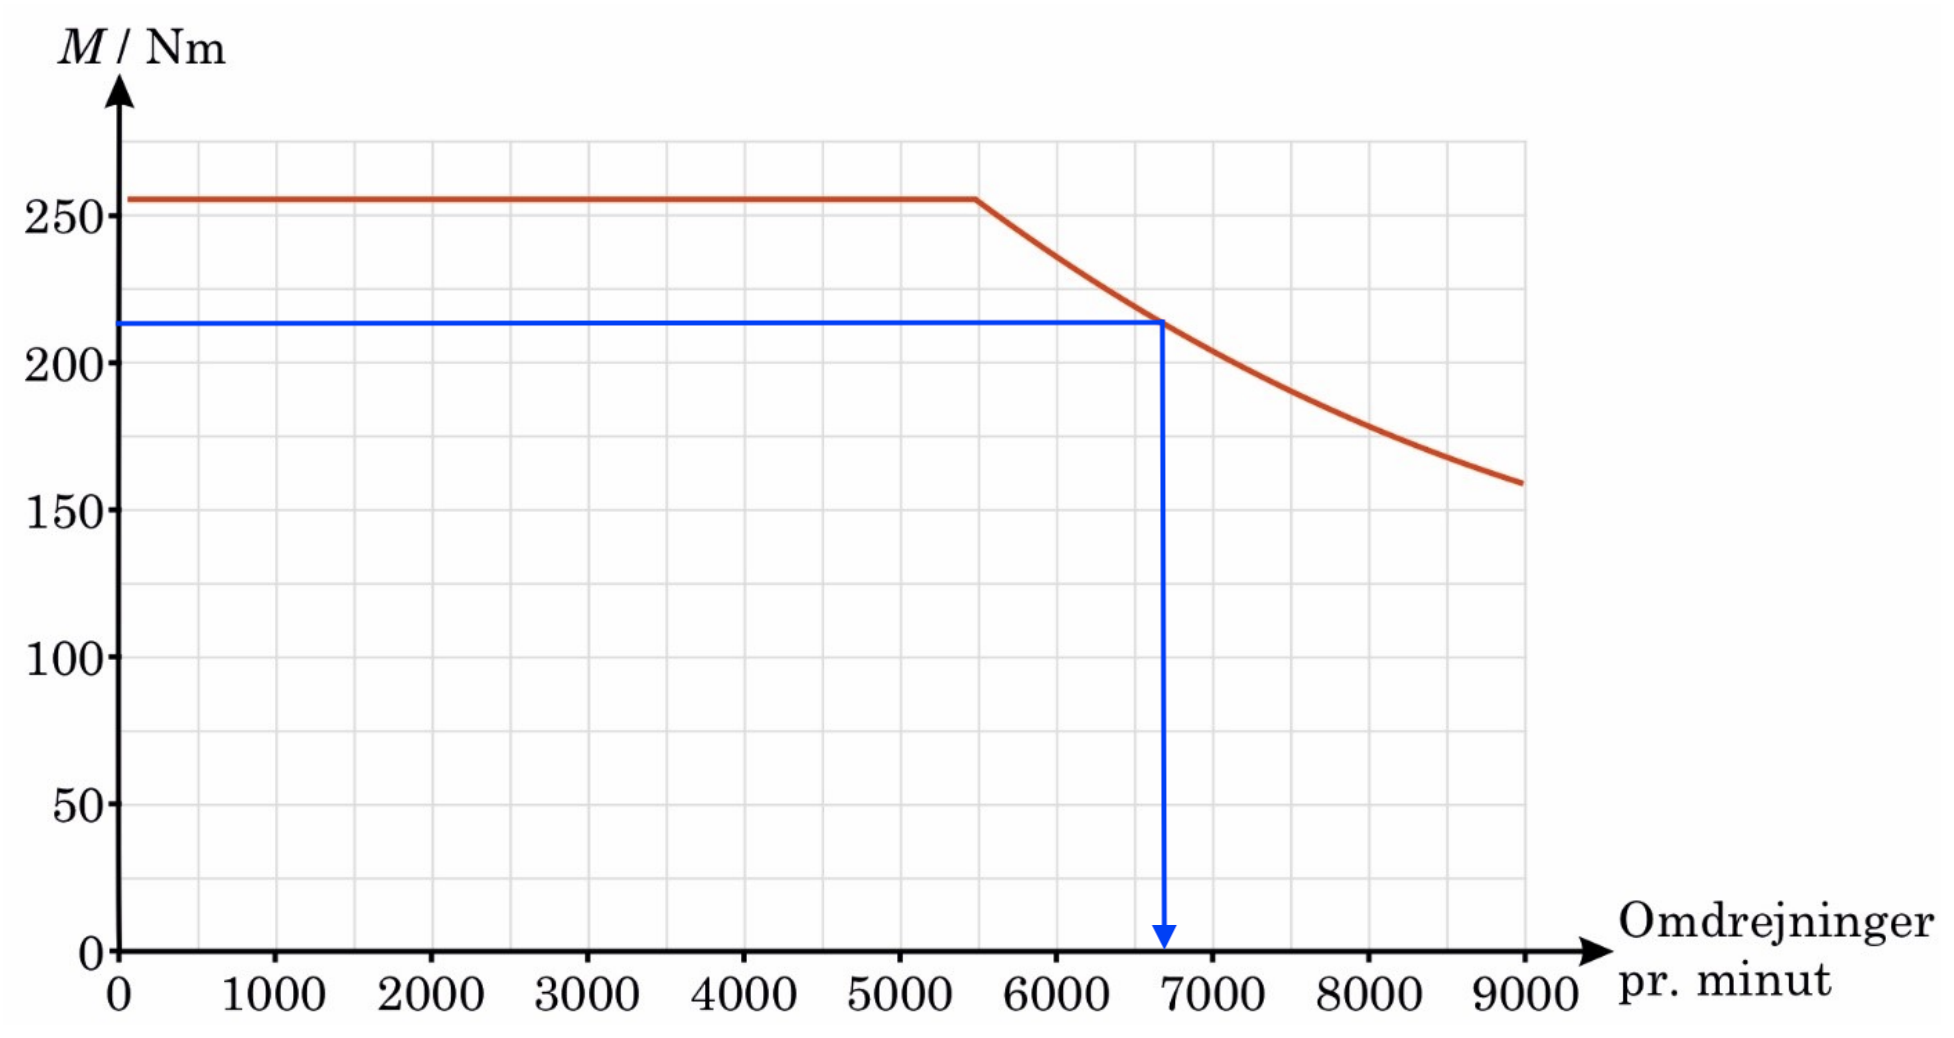
\includegraphics[width=\textwidth]{fM.png}
\end{center}
\caption{Aflæsning på grafen}
\label{fig:fM}
\end{figure}

\begin{question}{Batteri til elcykel}{}
  Et batteri er sat sammen af 220 enkelte Li-ion elementer.
  I batteriet er 20 elementer sat sammen i serie, og 11 sådanne serier er parallelforbundne i det samlede batteri.
Hvert element har indre resistans $40 \;\unit{m\ohm}$.
\begin{itemize}
  \item[a.] Beregn den indre resistans af det samlede batteri.
\end{itemize}
Hvert element har den maksimalt tilgængelige ladningskapacitet 2,56 Ah.
\begin{itemize}
  \item[b.] Beregn ladningskapaciteten af det samlede batteri i enheden Ah.
\end{itemize}
Et enkelt element undersøges ved at aflade det med den konstante strømstyrke 1,0 A.
Bilaget Batteri til elcykel indeholder sammenhørende værdier for spændingsfaldet $U$ over elementet, og den samlede ladning $Q$ der er løbet igennem elementet under afladningen.
\begin{itemize}
  \item[c.] Bestem den elektriske energi elementet afgiver under afladningen.
Bestem den gennemsnitlige effekt, hvormed elementet afgiver elektrisk energi under afladningen.
\end{itemize}
\end{question}
\sol \\
\textbf{a.}
Lad $R_{ie}$ betegne den indre resistans for et enkelt element. 
Siden det samlede batteri består af 11 parallelkoblede serier af elementer 20 elementer, så må den samlede indre resistans være
\begin{equation*}
\begin{split}
  R_i&=\frac{1}{11 \cdot \frac{1}{20 \cdot R_{ie}}}\\
  &=\frac{20}{11} \cdot R _{ie}\\
  &=\frac{20}{11} \cdot 40 \;\unit{m\ohm} \\
  &\approx 73 \;\unit{m\ohm}.
\end{split}
\end{equation*}
Den indre resistans af det samlede batteri er altså $73 \;\unit{m\ohm} $.\\[1ex]
\textbf{b.}
Det er åbenlyst, at ladningskapaciteten af et batteri er proportionalt med antallet af elementer.
Lad $n$ betegne antallet af elementer, så må ladningskapaciteten være
\begin{equation*}
\begin{split}
  Q _{\text{max} }&=n \cdot Q _{\text{element} }\\
  &=220 \cdot 2,56 \;\unit{Ah} \\
  &\approx 563 \;\unit{Ah}.
\end{split}
\end{equation*}
Ladningskapaciteten af det samlede batteri er altså $563 \;\unit{Ah} $. \\[1ex]
\textbf{c.}
Siden vi har
\begin{equation*}
\begin{split}
  \Delta E = \int_{t_1}^{t_2} U \,dQ, 
\end{split}
\end{equation*}
så må den elektriske energi, som aflades, svare til arealet under $(Q, U)$-grafen.
Denne bestemmes numerisk, hvilket ses i \cref{fig:QU}.
\begin{figure}[H]
\begin{center}
  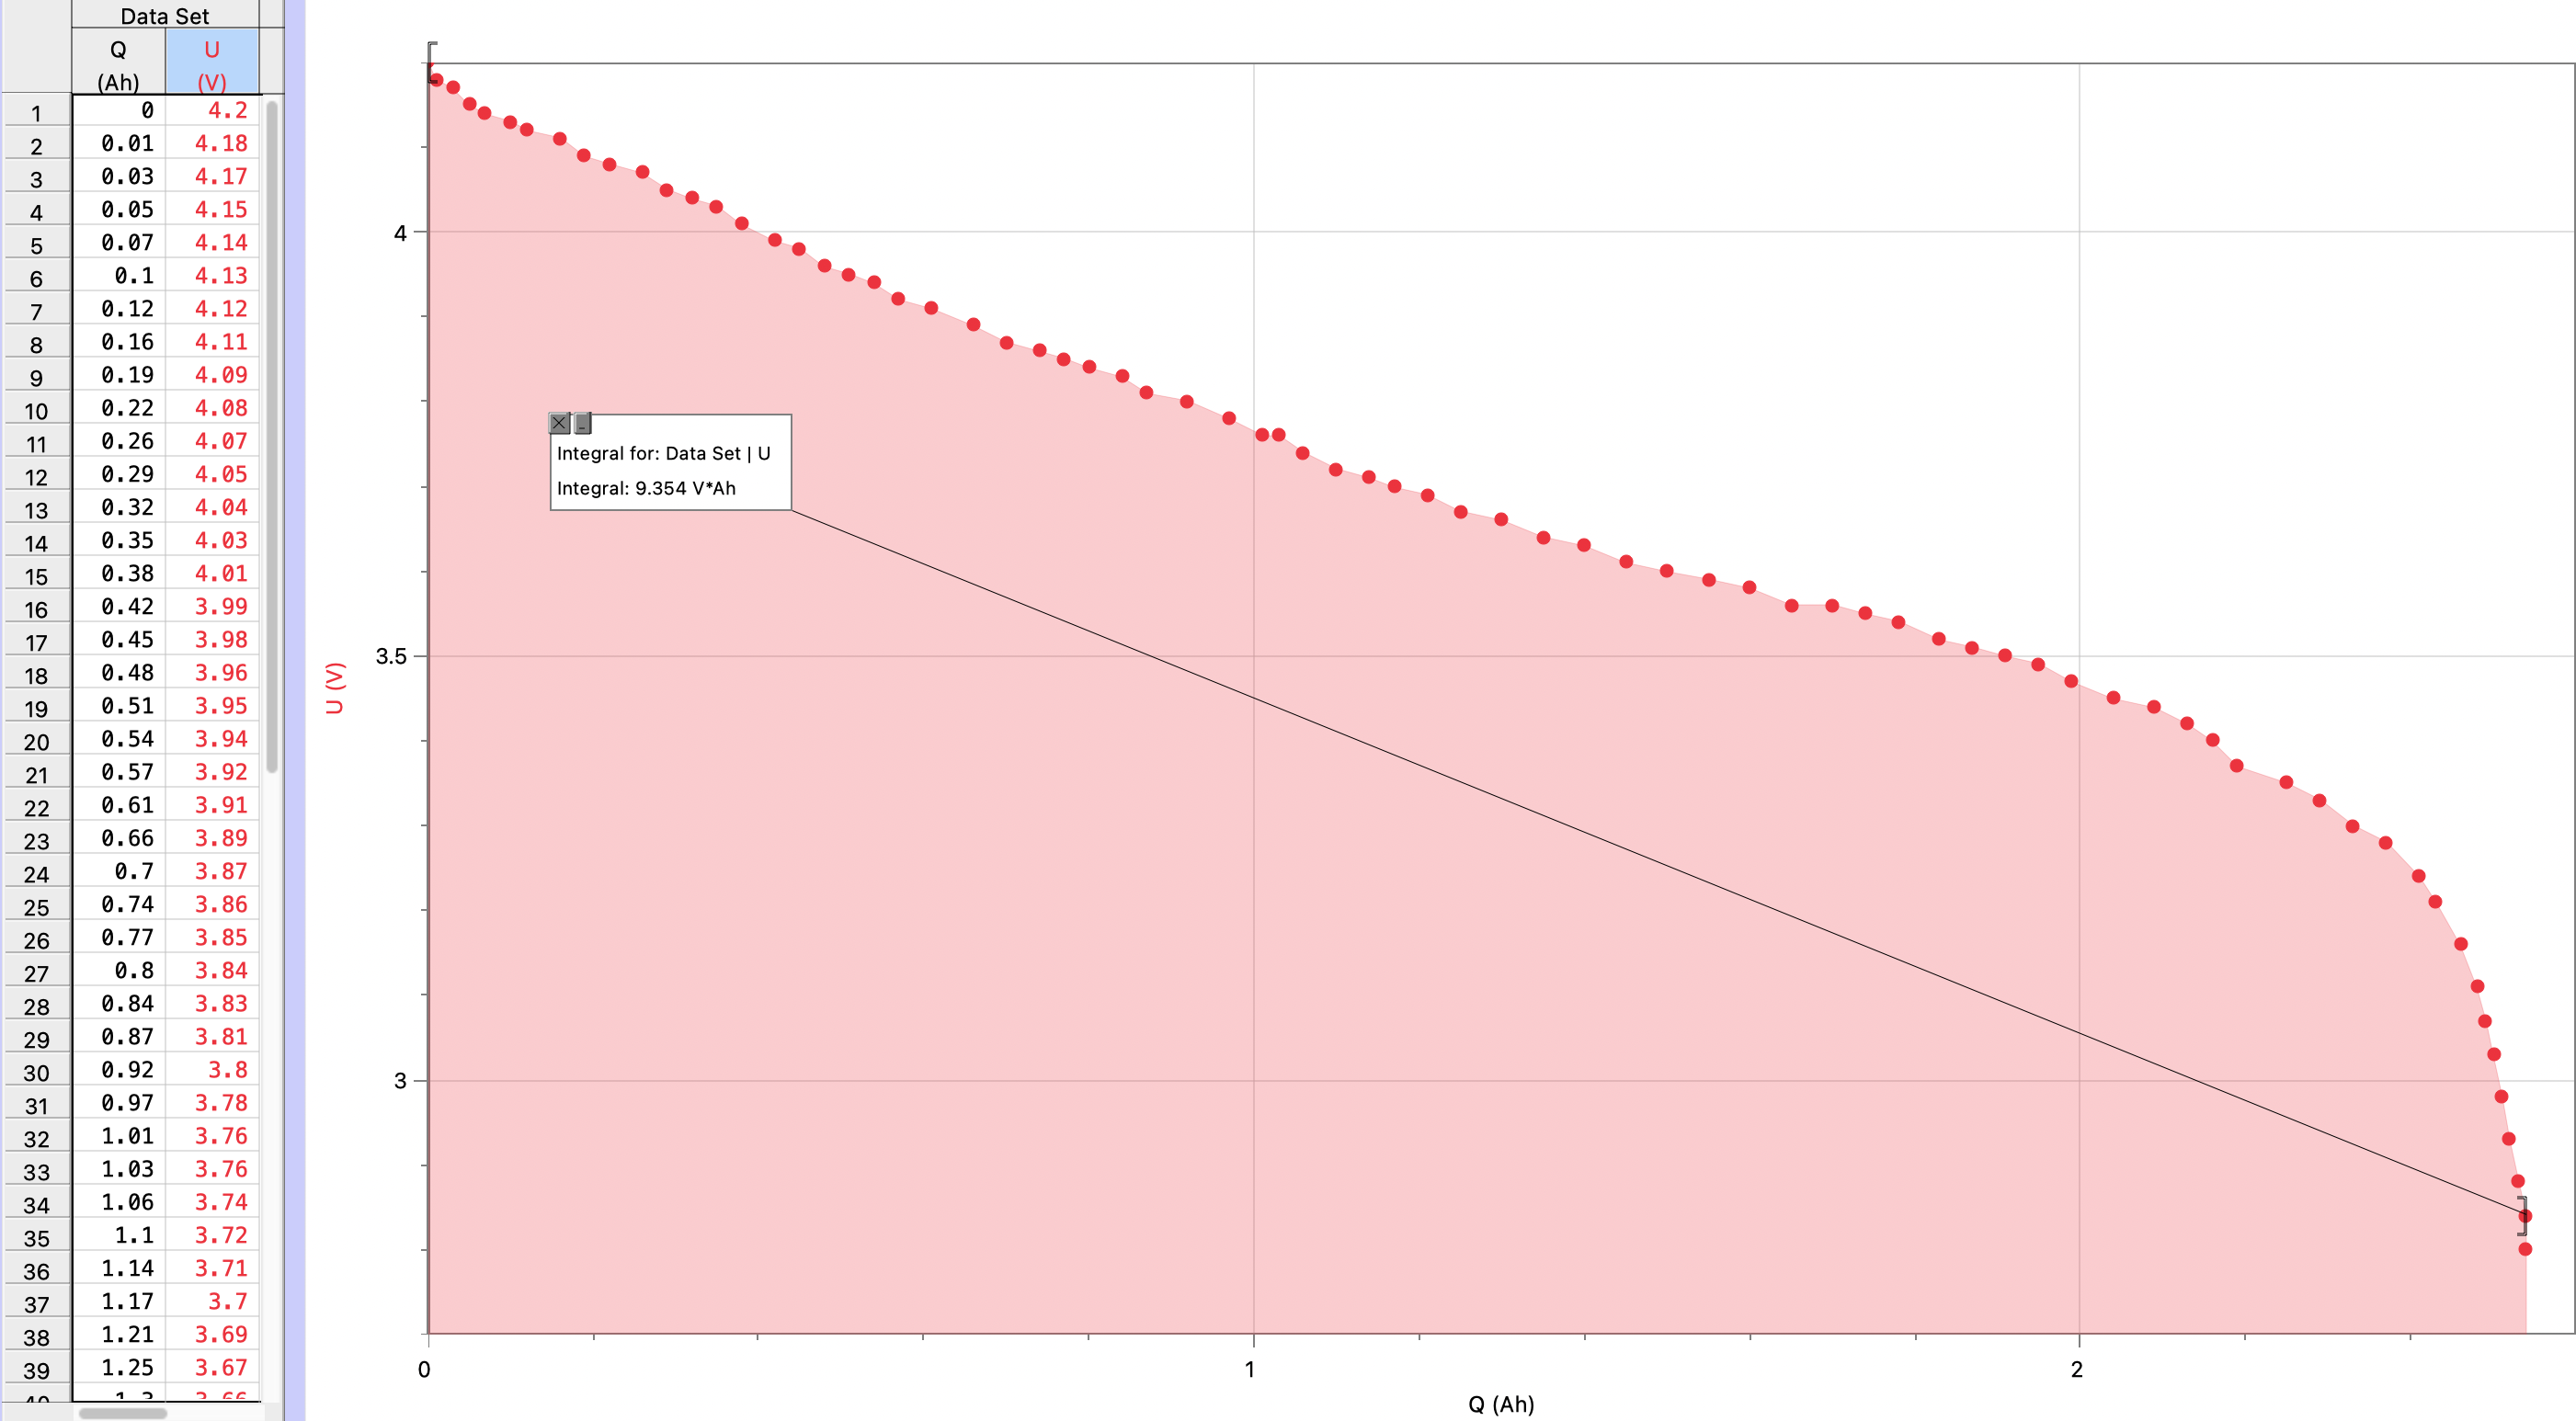
\includegraphics[width=0.8\textwidth]{QU.png}
\end{center}
  \caption{Numerisk integration på $(Q, U)$-grafen}
\label{fig:QU}
\end{figure}
Fra den numeriske integration har vi, at energien, der aflades, må være
\begin{equation*}
\begin{split}
  \Delta E&=9,354 \;\unit{V \cdot Ah} \\
  &=9,354 \;\unit{\frac{J}{C}} \cdot 3600 \;\unit{C} \\
  &\approx 3,37 \cdot 10^4 \;\unit{J} \\
  &=33,7 \;\unit{kJ}.
\end{split}
\end{equation*}
Den elektriske energi elementet afgiver under afladningen er altså $33,7 \;\unit{kJ} $.

Vi vil nu bestemme effekten, hvormed batteriet aflades.
Vi antager, at batteriet er fuldt opladet til start og bliver helt afladet under afladningen.
Så har vi
\begin{equation*}
\begin{split}
  SoC _{\text{efter} }= SoC _{\text{før} } - \frac{I \cdot \Delta t}{Q _{\text{max} }} &\iff 0=1-\frac{I \cdot \Delta t}{Q _{\text{max} }}\\
  &\iff \Delta t = \frac{Q _{\text{max} }}{I}.
\end{split}
\end{equation*}
Den gennemsnitlige effekt for afladningen må da være
\begin{equation*}
\begin{split}
  P &= \frac{\Delta E}{\Delta t} \\
  &=\frac{\Delta E \cdot I}{Q _{\text{max} }}\\
  &=\frac{33,674 \cdot 10^3 \;\unit{J} \cdot 1,0 \;\unit{A} }{2,56 \;\unit{A} \cdot 3600 \;\unit{s} } \\
  &\approx 3,7 \;\unit{W}.
\end{split}
\end{equation*}
Den gennemsnitlige effekt, hvormed elementet afgiver elektrisk energi under afladningen er altså $3,7 \;\unit{W} $.

\end{document}
